\documentclass[12pt,a4paper]{report}
\usepackage{parskip}
\usepackage[utf8]{inputenc}
\usepackage{amsmath}
\usepackage{amsfonts}
\usepackage{acronym}
\usepackage{amssymb}
\usepackage{graphicx}
\usepackage{chngcntr}
\usepackage{hyperref}
\usepackage[table]{xcolor}
\usepackage{glossaries}
\usepackage{caption}
\usepackage{booktabs}
\usepackage{algorithm}
\usepackage{subcaption}
\usepackage[hidelinks]{hyperref}
\usepackage{hyphenat}
%\usetikzlibrary{positioning}
\linespread{1.5}
\usepackage{mathptmx}
\usepackage{titletoc}
\usepackage{tocloft}
\usepackage{pgfkeys} 
\usepackage{listings}
\usepackage[english]{babel}
\usepackage{ragged2e}
\usepackage{setspace} \doublespacing
\usepackage[export]{adjustbox}
\usepackage{enumerate}
\usepackage[left=1in,right=1in,top=1in,bottom=1in]{geometry}
%\usepackage{lineno}
%\usepackage{cite}
%\usepackage{acronym}
\renewcommand{\baselinestretch}{1.5}
\usepackage[utf8]{inputenc}
\usepackage[dvipsnames]{xcolor}
\usepackage{tikz} 
\usetikzlibrary{shapes, arrows, positioning}
\usepackage{pgfgantt}
\usepackage{titlesec}
\usetikzlibrary{shapes.geometric,arrows}
\usepackage{natbib}


\setlength{\cftfigaftersnum}{\hspace{10pt}}

\usetikzlibrary{
	arrows,	calc,shapes,arrows,shapes.misc,shapes.arrows,chains,	matrix, 	positioning, scopes,	decorations.pathmorphing,	shadows, plothandlers,scopes,shapes.symbols,fit
}
\tikzstyle{startstop} = [ellipse, , minimum width=4cm, minimum height=1.2cm,text centered, draw=black,text width=3cm , rounded corners=0.5cm]
\tikzstyle{io} = [trapezium, trapezium left angle=70, trapezium right angle=110, minimum width=3cm, minimum height=1.2cm, text centered, draw=black,text width=3cm]
\tikzstyle{process} = [rectangle, minimum width=8cm, minimum height=1.2cm, text centered, draw=black  ]
\tikzstyle{process1} = [rectangle, minimum width=4cm, minimum height=1.2cm, text centered, draw=black  ]
\tikzstyle{decision} = [diamond, minimum width=7cm, minimum height=1.2cm, text centered, draw=black,aspect=2  ]


\tikzstyle{nodemcu} = [rectangle, minimum width= 3cm, minimum height= 4.5cm, text centered, draw = black, text width = 3cm]
\tikzstyle{blynkcloud} = [rectangle, minimum width= 3cm, minimum height= 8cm, text centered, draw = black, text width = 3cm]
\tikzstyle{sensor} = [rectangle, minimum width= 3cm, minimum height= 2cm, text centered, draw = black, text width = 2cm]
\tikzstyle{sensor1} = [rectangle, minimum width= 3cm, minimum height= 1cm, text centered, draw = black, text width = 2cm]

\usepackage{amsmath}
\usepackage{relsize}
\renewcommand{\cftfigfont}{Figure~}
\usepackage{tabularx}
\usepackage{multicol}
\usepackage{multirow}



\usepackage{sectsty}
\chaptertitlefont{\Large}
\sectionfont{\large}
\subsectionfont{\large}
\subsubsectionfont{\normalsize}
\paragraphfont{\normalsize}
\subparagraphfont{\normalsize}



\makeatletter

\usepackage[compact]{titlesec}  
\usepackage{times}






\titlespacing*{\subsection}{0pt}{1.5pt}{5pt}{ \fontfamily{times}}

\titleformat*{\subsubsection}{\centering \fontfamily{times}}
\titlespacing*{\chapter}{-2pt}{-20pt}{20pt}{ \fontfamily{times}}
\titlespacing{\section}{-2pt}{18pt}{5pt}{ \fontfamily{times}}


\titleformat{\chapter}[display]
{\normalfont\fontsize{16pt}{1.5pt}\selectfont\bfseries}{\chaptertitlename\ \thechapter}{0.5em}{\fontsize{16}{1.5pt}\selectfont\bfseries}

% Customize section headings
\titleformat{\section}
{\normalfont\fontsize{14pt}{1.5pt}\selectfont\bfseries}{\thesection}{0.5 em}{}

% Customize subsection headings
\titleformat{\subsection}
{\normalfont\fontsize{13pt}{2.5pt}\selectfont\bfseries}{\thesubsection}{0.5em}{}

	\captionsetup{skip=0pt}
\setlength{\belowcaptionskip}{0pt}

\setglossarystyle{list}
\makeglossaries
\newacronym{GPS}{GPS}{Global Positioning System}
\newacronym {GPRS}{GPRS}{General Packet Radio Service}
\newacronym{GSM}{GSM}{Global System for Mobile Communications}
\newacronym {IDE}{IDE}{Integrated Development Environment}
\newacronym{SMS}{SMS}{Short Message Service}
\newacronym{WHO}{WHO}{World Health Organization}







\begin{document}
	
	%------------------------------------Title Page--------------------------------------------------------	
	\begin{center}
		\large{
			\textbf{ \Large {KANTIPUR ENGINEERING COLLEGE} \\}
			\textbf{ (Affiliated to Tribhuvan University)\\ Dhapakhel, Lalitpur \\}
			\vfill
			
\includegraphics[width=0.3\textwidth]{kantipur.png} \\			
			\vfill
			\textbf{[Subject Code: EX 654]}
			\vfill
			\textbf{ A FINAL REPORT ON MINOR PROJECT\\ \large{"ACCIDENT DETECTION AND PREVENTION SYSYTEM"} }\\
\vfill
{\fontsize{14}{12}\selectfont \textbf{Submitted By:}}\\
\begin{tabular}{ll}
\textbf{Prabal Aryal} & \textbf{[33317]} \\
\textbf{Prabesh Raj Upadhaya} & \textbf{[33318]} \\
\textbf{Prakash Shrestha} & \textbf{[33319]} \\
\textbf{Subodh Pokhrel} & \textbf{[33327]} \\
\end{tabular}\\
\vfill
{\fontsize{14}{12}\selectfont \textbf{Submitted To:}}\\
	\large\textbf{Department of Computer and Electronics Engineering\\ Kantipur Engineering College }\\ 
				\textbf{\today}
			}
		}
	\end{center}
	\pagenumbering{gobble}
	
	%---------------------------------Abstract Page --------------------------------------------------	
	
	\pagebreak
\addtocontents{toc}{\protect\setlength{\cftbeforechapskip}{0pt}} % Adjust the value as needed
\addcontentsline {toc} {chapter} {Abstract}
\thispagestyle{plain}
\begin{FlushLeft}
 \textbf{\fontsize{16}{1.5pt}\selectfont Abstract}   
\end{FlushLeft}
\begin{justify}
This project entitled "Accident Detection and Prevention System" is based on the driver fatigue response system which alerts the driver whenever they feel drowsy and experience sleepiness during the drive. This project consists of an Eye Blink sensor which constantly monitors the eye of the driver and detects whether their eyes are closed for a certain period. In the case, that the eye has been closed for more than the threshold value, a warning buzzer along with vibration in the steering is generated for about 20 seconds before the system deduces there has passed out and an alert is sent to their specified relative via GSM modem using a text message.\\\\
This system will also contain a gas sensor that monitors the driver’s breath before and during the drive. If the driver is found to have consumed the alcohol, the engine will be abruptly stopped refraining from the control of the vehicle from the driver. Further, a vibration and gyro sensor shall be mounted on the system which alerts the driver’s relative through the same GSM modem sending a text message with the location of the vehicle on the condition an abnormal vibration and position has been detected and the driver is unable to notify the system that it is safe. All these systems and features will be controlled by an Arduino Uno microcontroller.\\   
        
\textbf{Keywords:} \textit {Accident Detection, , Alcohol Detection, Drowsiness Detection, Message Alert }
\end{justify}
		
	\pagenumbering{roman}
	
	
	%----------------------ACKNOWLEDGEMENT------------------------------------------------------------------------------
	\pagebreak
	\addtocontents{toc}{\protect\setlength{\cftbeforechapskip}{0pt}}
	\addcontentsline {toc} {chapter} {Acknowledgement}
	\thispagestyle{plain}
	

\begin{FlushLeft}
     \textbf{\fontsize{16}{1.5pt}\selectfont Acknowledgement}
\end{FlushLeft}
	\begin{justify}
    There are a lot of entities that are involved with the initiation and realization of every project. The entities may be as simple as a natural process, everyday events, and the people around us or something grand like a dream. These factors have undeniable importance and criticality in the realization of the projects and their initiation.\\\\
    Acknowledging such a role, it is vital that the entities responsible for building this project "Accident Detection and Prevention System" are thanked with utmost respect and gratitude. Primarily, the effort of the respected Head of Department of Electronics and Computer Engineering \textbf{Er. Rabindra Khati} and corresponding supervisor for the minor project \textbf{Er. Pralhad Chapagain}, \textbf{Er. Gopal Karn} and \textbf{Er. Sujin Gwachha} who provided much-needed guidance and a training environment for allowing the project to be conceived at the college level is much appreciated. The role of the respected teachers who have been with us through the times and have imparted invaluable knowledge, skill, understanding, and wisdom is of undeniable importance.\\
		
	\end{justify}
	\begin{FlushLeft}
		\textbf{Team Members:}	 \\
		Prabal Aryal \hspace{1.8cm}[33317]  \\
		Prabesh Raj Upadhaya \selectfont{ [33318]}\\
		Prakash Shrestha \hspace{1.1cm}\selectfont{[33319]}\\
        Subodh Pokhrel \hspace{1.3cm}\selectfont{[33327]}
	\end{FlushLeft}
	
	
	%---------------------------------------------TABLE OF CONTENTS  ------------------------------------------
	%----------------------------------------------------------------------------------------------
	%-----------------------------------------------------------------------------------------------
	\pagebreak
	\thispagestyle{empty}
	\addcontentsline {toc} {chapter} {Table of Contents}
	
	
	% Remove the page number and header from the table of contents
	\begin{center}
	

		\setlength{\cftbeforetoctitleskip}{0pt}

		\renewcommand{\contentsname}{\fontsize{16pt}{1.5pt}\selectfont\bfseries\textbf{TABLE OF CONTENTS} \fontfamily{times}}
		\setlength{\cftaftertoctitleskip}{2pt}
		\tableofcontents
	\end{center}
	
	
	
	
	
	%---------------------------------------------------------List of Figures---------------------------------------------
	
	\pagebreak
	
	
	
	\addcontentsline {toc} {chapter} {List of Figures}
	\thispagestyle{plain}

		\setlength{\cftbeforeloftitleskip}{0pt}

		\renewcommand{\listfigurename}{\fontsize{16}{1.5}\selectfont\bfseries\textbf{List of Figures}}
		%	\setlength{\cftbeforefigskip}{0pt}
			\setlength{\cftafterloftitleskip}{1.5pt}
		\listoffigures 
	
	
	%-------------------------------------------------------------------------List of Tables---------------------------------------------------
	\pagebreak
	\addcontentsline {toc} {chapter} {List of Tables}
	\thispagestyle{plain}
		\setlength{\cftbeforelottitleskip}{0pt}
	\renewcommand{\listtablename}{\fontsize{16}{1.5}\selectfont\bfseries\textbf{List of Tables}}
	\setlength{\cftafterlottitleskip}{1.5pt}
	\counterwithin{table}{chapter}
	
	\renewcommand{\cfttabpresnum}{Table\space}
	\cftsetindents{table}{0em}{4.5em}
		\listoftables

	
	
	
	\pagebreak
	%----------------------------------------------------Glossary of Acronyms---------------------------------------------
	\addcontentsline {toc} {chapter} {Abbreviations}
	\thispagestyle{plain}
	\begin{FlushLeft}
	    
		\textbf	{\Large {ABBREVIATIONS} \\}
	\end{FlushLeft}
		

	\begin{justify}
\textbf{GPS}:\hspace{0.5 cm}Global Positioning System\\
\textbf{GSM}:\hspace{0.3 cm} Global System for Mobile Communication\\
\textbf{IDE}:\hspace{0.6 cm}Integrated Development Environment\\
\textbf{SIM}:\hspace{0.5 cm} Subscriber Identity Module\\
\textbf{SMS}:\hspace{0.5 cm}Short Message Service\\
\textbf{WHO}:\hspace{0.3 cm}World Health Organization
	\end{justify}
	
	
	
	% Print the acronym list
	
	
	
	
	%	\printacronyms
	
	
	
	%------------------------------------------------------Chapter 1 Introduction ---------------------------------------------

	\addtocontents{toc}{\protect\setlength{\cftbeforechapskip}{16.5pt}}
 	\chapter {INTRODUCTION}
	\pagenumbering{arabic}
	
	\section{Background}
	
	\begin{justify}

According to the World Health Organization (WHO), approximately 1.3 million fatalities occur annually due to traffic road crashes, making vehicle accidents one of the foremost causes of mortality worldwide. Despite efforts to mitigate these occurrences, accidents remain inevitable; however, the timely provision of assistance to accident victims can significantly reduce the associated loss of life. It is imperative to address the issue of unnoticed accidents by promptly notifying rescue authorities and relevant contacts about such incidents. Therefore, the primary aim of this project is to develop a system capable of automatically detecting accidents and promptly alerting designated individuals or authorities to facilitate timely intervention, thereby minimizing casualties.\\\\
The proposed system relies on the integration of various components, including a GPS and GSM module, within an Arduino Uno platform. Key to its functionality is a gyroscope sensor module, which detects changes in vehicle axes indicative of an accident. Upon detection, the system generates an automated message containing precise accident location data, which is then transmitted to predefined contacts or rescue authorities, contingent upon the severity of the incident.\\\\
By implementing such a system, it is envisaged that the prompt dissemination of information regarding accidents will enable swift response efforts, ultimately contributing to a reduction in the loss of life resulting from road traffic crashes.
	\end{justify}
	
	
	%---------------------------------------------------------------------Problem Statement--------------------------------------------------------------------
	
	\section{Problem Statement}
	
	\begin{justify}
Various inquiry reports of road accidents issued by WHO were studied and it was seen that most of the road accidents result from the carelessness of the rider and a large toll of people were due to delays in the rescue of the involved. This accident detection and prevention system helps prevent such accidents by meticulously preventing the driver from drinking and driving and falling asleep during the ride as well as informing the nearby hospital and victim's family member about the accident which increases the chances of survival to a degree.
	\end{justify}
	
	%	---------------------------------------------------------------
%-Objective-------------------------------------------------------------------
	\section{Objective}
	
	\raggedright
	{ The main objectives of this project are: \\
		\begin{itemize}
			%	\setlength\itemsep{0.5em}
				\setstretch{1}
			\item To holistically enhance road safety by integrating real-time accident detection, early warning systems, and automated emergency response systems.
		\end{itemize}
	}
	\section{Application}
 \raggedright
 {
 Like every other project, this proposed project is designed in such a way that it has some significant applications.
\begin{itemize}
    \item 	Monitor drowsiness and alcohol consumption before and during the drive.
    \item Locate the vehicle as fast as possible.
    \item Can be used in smart cities to maintain traffic regulations. 
\end{itemize}
 }

	%--------------------------------------------------------------Project Features------------------------------------------------------------------
	\section{Features}
	
	\raggedright
	{ Some features of this project are: \\
		\begin{itemize}
				\setstretch{1}
			%	\setlength\itemsep{0.5em}
			\item Provide messages automatically to the concerned authorities or close contacts in case of an accident.
    \item 	Apply several precautionary methods to mitigate accidents.	
			
		\end{itemize}
	}
	
	%-------------------------------------------------------------------Feasibility Analysis--------------------------------------------------------------------
	\section{Feasibility Analysis}
 There were two types of feasibility studies to which the system was subjected, as described below. The key considerations involved in the feasibility study are described below:
\vspace{0.75cm}
	\subsection{Technical Feasibility}
	
	\begin{justify}
The system consists of electronic components like Arduino Uno, and GSM modules along with sensors like gas sensor and eye blink sensor. These components operate at low voltage so there are no electrical risks. The software used in this project can be easily learned and is user-friendly.
	\end{justify}
	
	\subsection{Economic Feasibility}
	
	\begin{justify}
		We must analyze whether the project is economically feasible or not by comparing the cost required to develop the project, integrate it with the system, and operate the system with benefits that are achieved using the product i.e., we perform the cost benefits analysis for the purpose. This system is affordable since it uses simple modules so This project can be economically feasible.
	\end{justify}
	

	
	%-----------------------------------------------------------------------------Literature Review ----------------------------------------------------------------------------------------------------
	\chapter{LITERATURE REVIEW}
	
	\begin{justify}
The system that detects and notifies road accidents has been designed and developed for a very long time now. The paper below has presented summaries of different past attempts which were made to develop systems related to accident detection and alert using various technologies.\\\\
Dr. R. Prasanthi, M.U. Nitish Babu, B. Jaswanth, and G. Sumith Chandra's study \cite{Prasanthi2023} researched accident detection and alert system addressing unattended accidents among vehicle riders. The system, integrating Arduino, GPS Receiver, and GSM module, employed GPS for vehicle direction and GSM for sending SMS alerts to contacts with directional information and Google Maps links. It features Vibration sensor-based severe accident detection and rollover identification. The microcontroller transmits data to the GSM module, relaying victim location to contacts for swift aid using GPS MODEM. This research significantly enhances road safety, offering an advanced solution for timely assistance in vehicular accidents, particularly impactful in regions like Nepal, India, and Bangladesh.\\\\
C. K. Gomathy, K. Rohan, B. Mani Kiran Reddy, and V. Geetha \cite{Gomathy2021} proposed a solution centered on automatic accident detection and alert systems. The primary aim is to enhance accident control by employing wireless communication methods to promptly notify registered mobiles, hospitals, and police stations. In cases of accidents occurring within cities or areas, a GSM module expedites message transmission to registered mobiles. The heart of the system lies in Arduino, facilitating seamless communication across devices. Triggered by accident-induced vibrations, the system swiftly transfers information via GSM to registered numbers. The GPS is pivotal in locating the accident site. This proposed approach verifies accident occurrences, instantly notifying nearby medical facilities and registered mobiles through GSM and GPS modules. Geographical coordinates are transmitted via a tracking system. The study underscores the significance of the vibration sensor as a major module for detecting accidents.\\\\
            D. S. Aarya, C. K. Athulya, P. Anas, B. Kuriakose, J. S. Joy, and L. Thomas \cite{Aarya2018} proposed a system that states vehicle accidents are one of the leading causes of fatality. The period between the occurrence of an accident and the dispatch of emergency medical services to the accident site is a critical factor in accident survival rates. Accident detection and messaging systems will be stationed in vehicle itself which will be helpful during the time of accident as hospital, police and emergency contact can be informed immediately. The system is executed using GPS and GSM technology. A vibration sensor detects a collision using piezoelectric effect, which is the ability of certain materials to generate an electric charge when they are under mechanical stress. As soon as the collision is detected the GPS module locates the accident (latitude and longitude) and sends a message to the hospital and the emergency contact using the GSM module. The ambulance arrives to the location which is tracked by the GPS module and hence the victim is treated as soon as possible reducing the help time. In case if there is a minor accident, the victim can press a switch (button) to prevent the emergency contacts from being alerted. This system comprises of Arduino, GPS, GSM and vibration sensor, which detects the accident and alerts the authorities immediately, it also combats false alarms by using a switch provided for the driver.\\\\
            R.Saranya, R.Arun Kumar propose a system that helps prevent vehicle accidents using sensors \cite{Saranya2017}. Accidents may vary in different positions and it can be done through sleepiness or a third party. To avoid these
types of accidents we introduce the alert system by using
different types of sensors. It consists of two types one is
a transmitter and the other is the receiver. The transmitter sends
the rays to the eye. If our eye is closed, then the output will be
increased. If the eye is open, then the output is decreased.
The output is set like an alarm that is located inside the
vehicle. It will go on for some time until the driver is
back to his senses. If the driver can’t have any control within
the time, then the alarm outside the vehicle will give an alert to
the driver. There may be a case that the vehicle can meet
with an accident. In such a situation, an alert will be sent to the
nearest hospital.\\\\
            While extensive research has been conducted on Accident Detection and Prevention Systems, the existing literature predominantly emphasizes the utilization of a vibration sensor with digital output and the SIM module operating on a 2G signal. This paper seeks to address a research gap by focusing on optimizing the overall system. Our approach involves incorporating an analog vibration output sensor and upgrading the communication module to 4G SIM technology. This novel aims to enhance the efficiency and effectiveness of accident detection and prevention systems, providing a valuable contribution to the existing body of research in this field.
        \end{justify}
	
	
	
	%------------------------------------------------------------------------------------------System Requirements--------------------------------------------------------------------------------------------
	\chapter{SYSTEM REQUIREMENTS}
%--------------------------------------Hardware Requirement ----------------------------------------------------------
	\section{Hardware Requirement}
	\subsection{Arduino}
	\begin{justify}
Arduino UNO is a type of Arduino board that is provided as an open board that uses an ATmega328p microcontroller in the board. The Arduino Uno contains a set of analog and digital pins that are input and output pins that are used to connect the board to other components. The board has a USB connection that can be used to give a power supply to the board. The board is used for electronics projects and used to design the circuit. In this system, it serves as a versatile platform for data acquisition, processing, and triggering early warnings and communication for emergency response.
		\end{justify}
 \begin{figure}[ht]
     \centering
     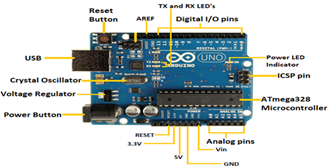
\includegraphics[width=0.5\textwidth]{Picture1.png}\\
     \caption{{Arduino}}
     \label{fig:enter-label}
     	\Source{[https://www.reichelt.com/de/en/arduino-uno-rev-3-atmega328-usb-arduino-uno-p119045.html?GROUPID=6667&&r=1]}
 \end{figure}
	
	\subsection{Gas Sensor}
	\begin{justify}
The MQ-3 gas sensor is a low-cost, alcohol-sensitive sensor that can detect the presence of alcohol vapors in the air.  This system, is primarily used to identify potential driver intoxication. If the MQ-3 sensor detects high levels of alcohol, the system triggers warnings to the driver and prevents the vehicle from starting, helping to reduce the risk of accidents caused by drunk driving consumption. 
	\end{justify}
	\begin{figure}[ht]
	    \centering
	    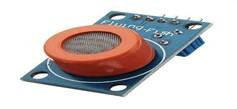
\includegraphics[width=0.4\textwidth]{Picture3.jpg} 
	    \caption{Gas Sensor}
      \Source{[https://pricemandu.com/products/alcohol-level-sensor-mq3-53dfe7dd9aa2004908140117fc8d8f73/]}
	    \label{fig:enter-label}
	\end{figure}
	
	
	%-------------------------------------
	
	
	\subsection{Vibration Sensor}
	\begin{justify}
The Minisense 100 from Measurement Specialties is a low-cost cantilever-type vibration sensor loaded by a mass to offer high sensitivity at low frequencies. Useful for detecting vibration and 'tap' inputs from a user. A small AC and large voltage (up to +/-90V) are created when the film moves back an forth. A simple resistor should get the voltage down to ADC levels. Can also be used for impact sensing or a flexible switch. In this system, it detects the impact on the vehicle.
\end{justify}
	\begin{figure}[ht]
	    \centering
	    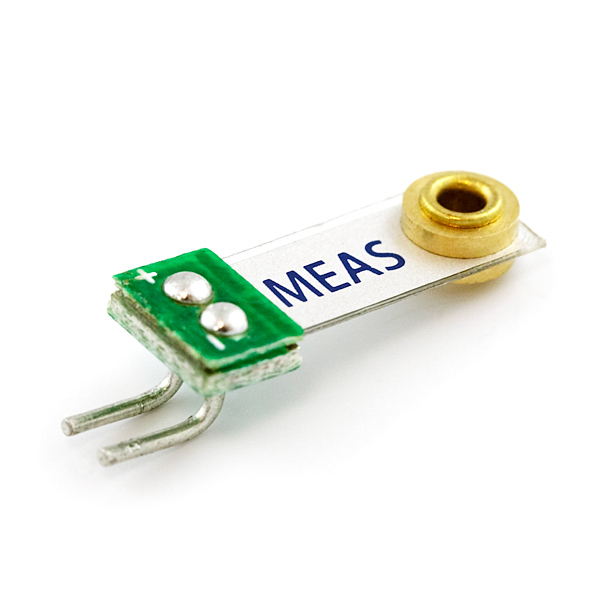
\includegraphics[width=0.4\textwidth]{09199-03-L.jpg}
	    \caption{MEAS Vibration Sensor}
     \Source{{https://www.sparkfun.com/products/9199}
	    \label{fig:enter-label}
	\end{figure}
	
	%-------------------------------------
	
	\subsection{GSM Module}
	\begin{justify}
SIM 900A offers GSM technology for communications with the use of a mobile sim. It uses a 900 and 1800MHz frequency band and allows users to send/receive mobile calls and SMS. It also has modes, command mode, and data mode. Also, the keypad and display interface allows the developers to make customized applications within it. It is used for sending messages in case of accident occurs in this system. 	
	\end{justify}
	\begin{figure}[ht]
	    \centering
	    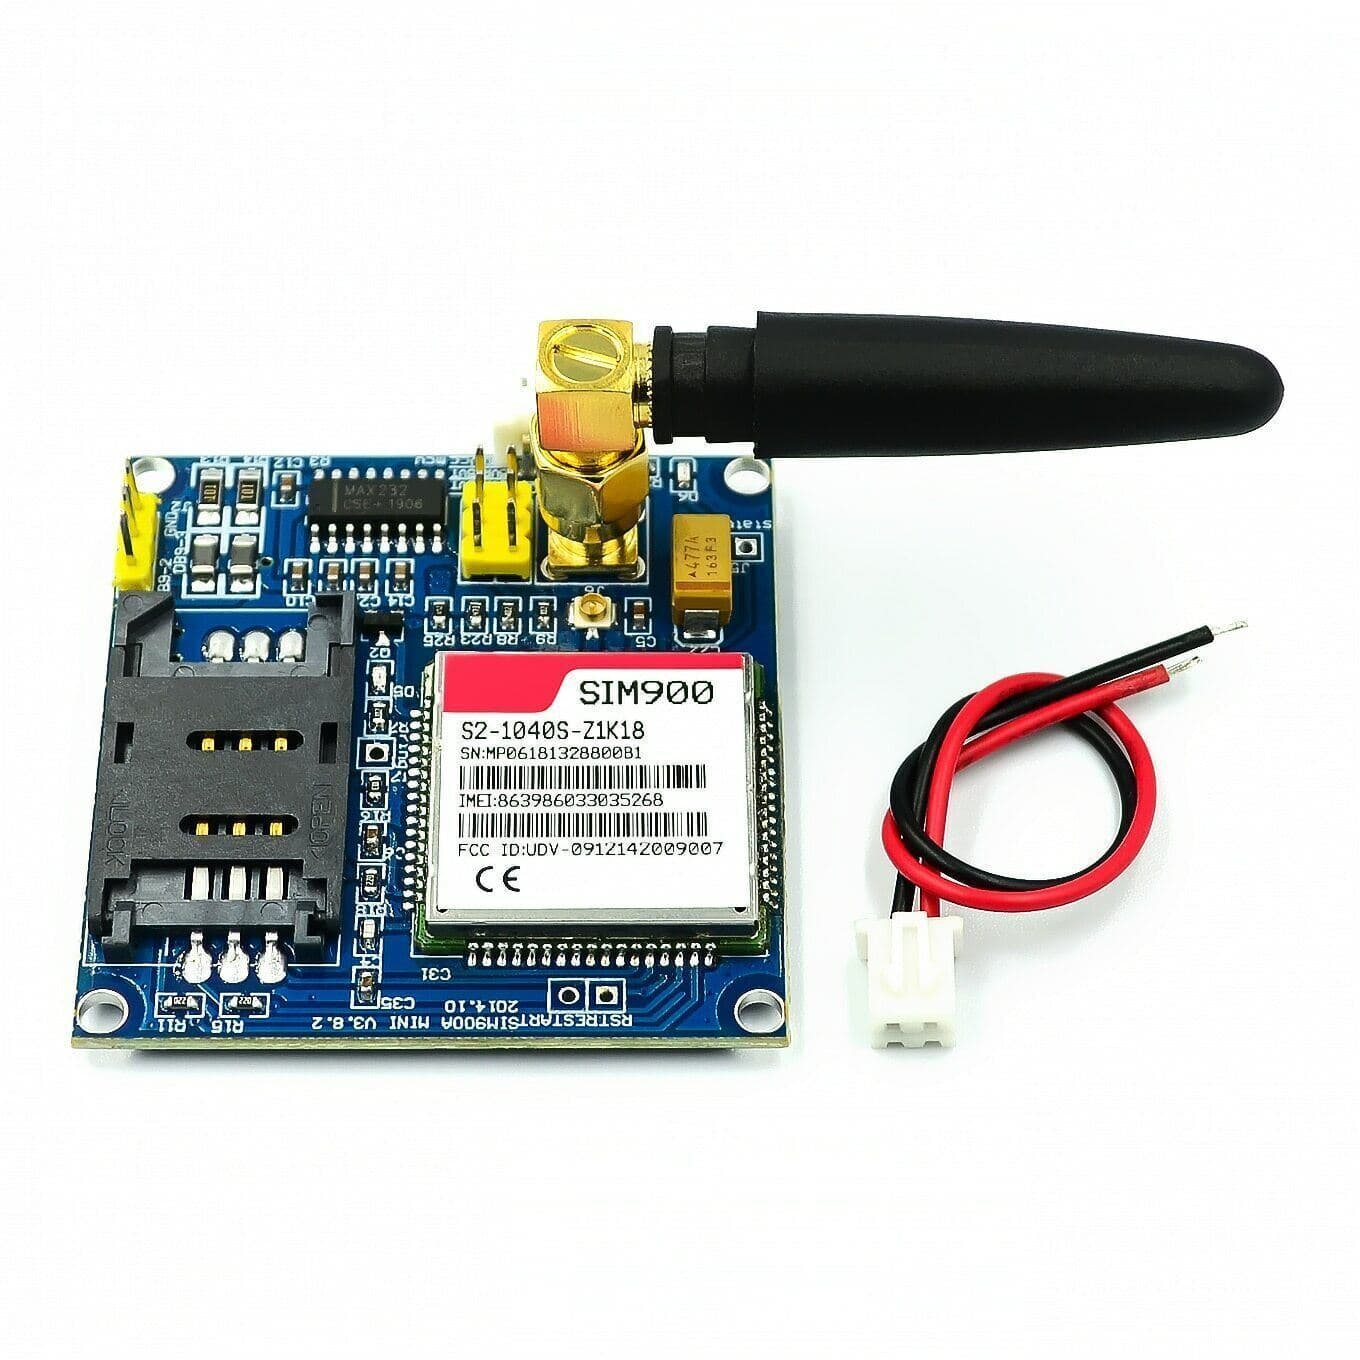
\includegraphics[width=0.5\textwidth]{sim.jpeg}
	    \caption{SIM 900a}
     \Source{[https://forum.arduino.cc/t/sim900a-network-connection-problem/1169263]}
	    \label{fig:enter-label}
	\end{figure}
	
	%-------------------------------------
	
	\subsection{Gyroscope Sensor}
	\begin{justify}
		A gyroscope sensor is a device that measures or maintains orientation and angular velocity. It is a spinning wheel or disc in which the axis of rotation (spin axis) is free to assume any orientation by itself. When rotating, the orientation of this axis is unaffected by tilting or rotation of the mounting, according to the conservation of angular momentum. It detects the roll and pitch of the vehicle in this system.
	\end{justify}
	\begin{figure}[ht]
	    \centering
	    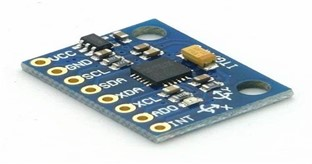
\includegraphics[width=0.3\textwidth]{Picture6.jpg}
	    \caption{MPU6050 Gyroscope Sensor}
     \Source{[https://images.app.goo.gl/3qsKHTHPJ1VHARQA8]}
	    \label{fig:enter-label}
	\end{figure}
	
	%-------------------------------------
	\subsection{Eye Blink Sensor}
	\begin{justify}
	
Eyeblink sensors utilize infrared technology to detect when someone closes their eyes. They emit an invisible beam of light that bounces back to a receiver when your eyes are open. When you blink, the reflection drops significantly, indicating a closed eye. In this system, it is used to identify drowsiness, a major risk factor in accidents. The sensor monitors blinking patterns and compares them to established baselines of alert driving.
	\end{justify}
	\begin{figure}[ht]
	    \centering
	    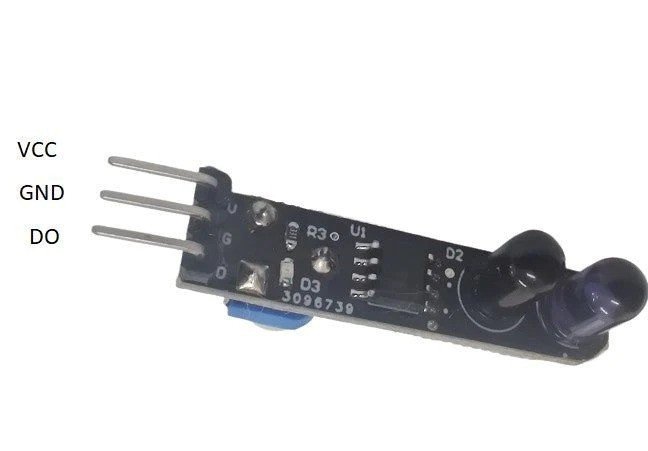
\includegraphics[width=0.3\textwidth]{viber_image_2024-02-29_07-41-30-340.jpg}
	    \caption{Eye Blink Sensor}
     \Source{[https://robocraze.com/products/eye-blink-sensor]}
	    \label{fig:enter-label}
	\end{figure}
	\subsection{GPS Module}
 \begin{justify}
     The NEO-6M GPS module is a compact that enables accurate location tracking. In accident detection and prevention systems, it determines the exact location of a vehicle accident. This information is critical for several reasons: it allows emergency services to be dispatched quickly and precisely to the site, ensuring rapid assistance for anyone injured. The NEO-6M, specifically, is commonly used because it's cost-effective, highly sensitive for reliable signals, and integrates well with microcontrollers typically used in these systems.  
 \end{justify}
 \begin{figure}[ht]
     \centering
     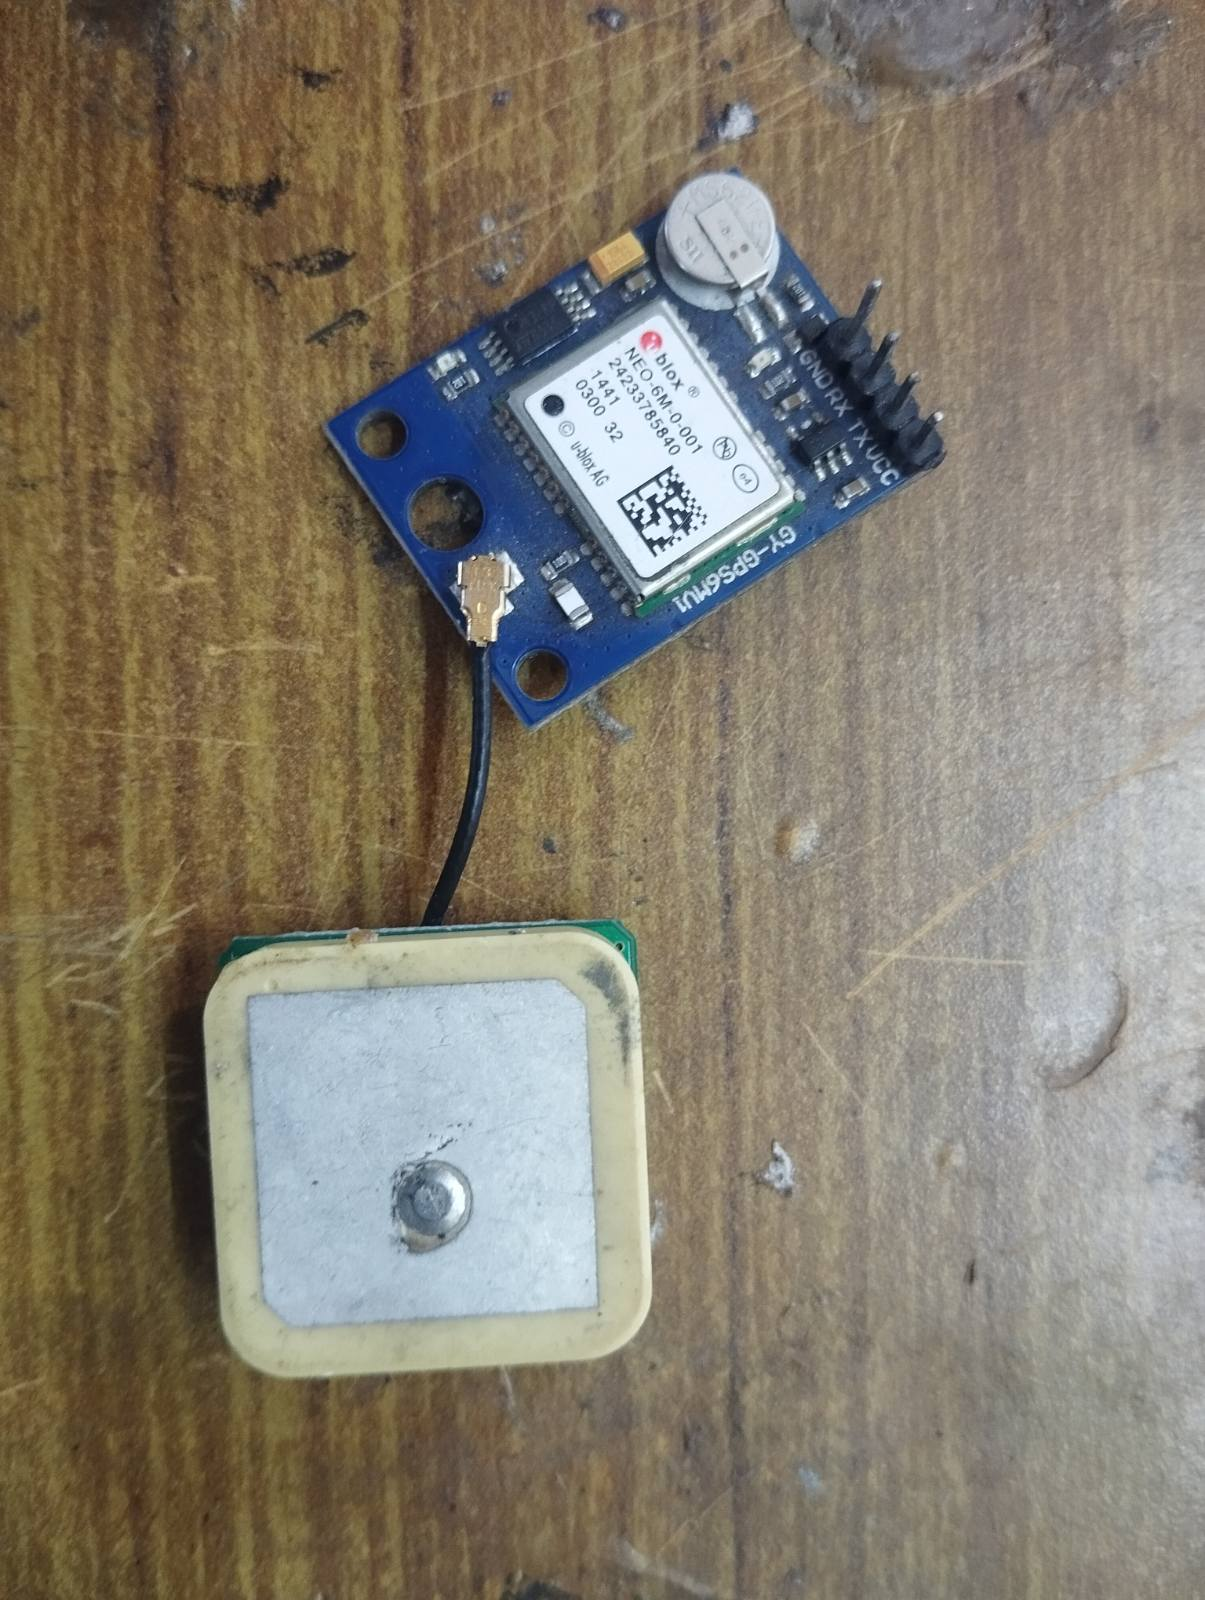
\includegraphics[width=0.3\textwidth]{viber_image_2024-02-29_13-26-11-103.jpg}
     \caption{NEO-6M}
     \label{fig:enter-label}
 \end{figure}
	%-------------------------------------

		
	\section{Software Requirements}
	
	\subsection{Arduino Software (IDE)}
	
	\begin{justify}
		The Arduino IDE (Integrated Development Environment) is a software platform specifically designed for programming Arduino microcontroller boards. It provides a user-friendly interface that simplifies the process of writing, compiling, and uploading code to Arduino boards. The IDE is open-source and available for multiple operating systems, including Windows, macOS, and Linux. It uses a simplified version of the C++ programming language, making it accessible to beginners and experienced developers alike. \\ 
		\\In the Arduino IDE, users can write code using the familiar setup() and loop() functions, where setup() is executed once during the board's initialization, and loop() runs repeatedly as long as the board is powered on. The IDE comes with a vast library of pre-written functions and examples, enabling users to quickly incorporate various functionalities into their projects without starting from scratch. The IDE also offers a serial monitor, allowing users to interact with their Arduino board and debug code by sending and receiving data in real-time. Overall, the Arduino IDE serves as a fundamental tool for the Arduino ecosystem, empowering hobbyists, students, and professionals to unleash their creativity and build a wide range of projects, from simple blinking LED circuits to complex robotics and IoT applications.
	\end{justify}	
			
	%-------------------------------------
	
	
	
	
	%-------------------------------------
	
	
	
	
	
	
	%-------------------------------------------------------chapter 4 methodology --------------------------------------------------------------------------------------
	\chapter{METHODOLOGY}
 \begin{justify}
     
	Accident Detection and Alert System is designed to reduce accident fatalities. This system prioritizes the real-time detection and alerts of the accident to the emergency service provider so that many lives can be saved.\\\\
This system comprises various sensors that ensure the safety of the driver, passengers, and other vehicles on the road. The first is an MQ3 gas sensor that continuously measures the driver's breath for the presence of alcohol vapor. If it detects levels beyond the set threshold, it triggers the relay to stop the vehicle. The second sensor is a MEAS vibration sensor that monitors the vibrations felt by the vehicle. If it senses excessive vibrations beyond the threshold level, it instantly cuts the power supply to the engine and triggers the documentation process. The system also includes a sensor that continuously monitors the orientation of the vehicle. If it detects the vehicle's orientation to be beyond the set threshold, it alerts the predefined contact number with the documentation details. Additionally, the system features an Eye Blink sensor that detects drowsiness in the driver. If the driver is asleep, the sensor triggers a buzzer to alert them before stopping the vehicle. In the event of an accident, the system sends information about the accident along with the geo-location to the predefined contact number.
 \end{justify}
\newpage
	\section{Hardware Development}
\subsection{Block Diagram}
\begin{figure}[ht]
    \centering
	\begin{tikzpicture}[auto, node distance=2cm,>=latex']
    % Define block styles
    \tikzstyle{block} = [rectangle, draw, text width=5em, text centered, rounded corners, minimum height=4em]
    \tikzstyle{line} = [draw, -latex']
    
    % Nodes
    \node [block] (vibration) {Vibration Sensor};
    \node [block, below of=vibration] (gas) {Gas Sensor};
    \node [block, below of=gas] (blink) {Blink Sensor};
    \node [block, below of=blink] (gyro) {Gyroscope Sensor};
    \node [block, right of=gas, node distance=10cm,minimum size=4cm] (arduino) {ARDUINO UNO Microcontroller};
    \node [block, below=1cm of arduino] (gsm) {GSM/GPS Module};
    \node [block, below=1cm of gsm] (smartphone) {Smartphone};
    \node [block,above=1cm of arduino](power) {Power Supply}
    
    % Arrows
    \path [line] (vibration) -- (arduino);
    \path [line] (gas) -- (arduino);
    \path [line] (blink) -- (arduino);
    \path [line] (gyro) -- (arduino);
    \path [line] (gsm) -- (arduino);
    \path [line] (gsm) -- (smartphone);
    \path [line](power) -- (arduino)
\end{tikzpicture}
   \caption{Block Diagram}
    \label{fig:enter-label}
   
    
\end{figure}
 
    \begin{justify}
        The accident detection and prevention system comprises a set of sensors, including a vibration sensor for impact detection, a gas sensor for alcohol detection, a blink sensor to monitor driver drowsiness, and a gyroscope sensor for the spatial orientation of the vehicle. These sensors are interfaced with an Arduino Uno microcontroller, which serves as the central processing unit.\\\\
        Upon receiving input from the sensors, the Arduino Uno analyzes the data and executes predefined actions based on the detected conditions. For instance, if an impact is detected or the vehicle rolls over, the system can trigger emergency messages or alerts. Similarly, it can activate alarms or warning systems to notify the driver or nearby individuals.
    \end{justify}
	\pagebreak    
	\section{Software Development}
	\subsection{Flowchart}
 \begin{justify}
     The flowchart likely represents a safety system for a vehicle. It probably starts with initializing sensors, and then takes readings from multiple sensors like a gas sensor, eye blink sensor, and others.  Arrows likely connect these steps to diamonds representing decisions about whether sensor readings exceed certain thresholds. Based on these decisions,  the system might start the engine, ring a buzzer, check GPS location,  or ultimately stop the vehicle.
     \vspace{5cm}
     	\begin{table}[h]
\centering
\caption{Threshold Values}
\label{tab:sensor_info} % Optional: Add a label for referencing the table
\begin{tabular}{|p{3cm}|p{3cm}|p{9cm}|}
\hline
\textbf{Sensor Name} & \textbf{Threshold Value} & \textbf{Source} \\ \hline
Vibration & 4 V & [https://www.irjet.net/archives/V4/i10/IRJET-V4I10162.pdf] \\ \hline
Gyroscope & 90 degrees & An Accident Detection and Classification System Using Internet of Things and Machine Learning towards Smart City  \\ \hline
MQ3 Gas & 300 ppm & [https://www.who.int/initiatives/SAFER/drink-driving] \\ \hline
Eye Blink & 4 second & [https://www.irjet.net/archives/V4/i10/IRJET-V4I10162.pdf]\\ \hline
\end{tabular}
\end{table}
       \end{justify}
 \begin{figure}[h]
\begin{center}
\begin{adjustbox}{width=\textwidth,height=\textheight}
\begin{tikzpicture}[
    scale=0.6,transformshape,
    startstop/.style={ellipse, minimum width=2.5cm, minimum height=1.5cm,text centered, draw=black},
    io/.style={rectangle, minimum width=2.5cm, minimum height=1.5cm, text centered, draw=black},
    decision/.style={diamond, minimum width=2cm, minimum height=1.5cm, text centered, draw=black,aspect=5},
    process/.style={rectangle, minimum width=2cm, minimum height=1cm, text centered, draw=black},
    arrow/.style={thick,->,>=stealth},
]
% Define nodes
\node (start) [startstop] {Start};
\node (in1) [io, below=0.1cm of start,yshift=-0.5cm] {Initialize threshold value of all sensor};
\node (in2) [io, below =0.1cm of in1, yshift=-0.5cm] {Get value from gas sensor};
\node (dec1) [decision, below of=in2, yshift=-1cm] {Is value $>$ threshold};
\node (stop1) [startstop, right of=dec1,xshift=6cm] {Stop vehicle};
\node (pro1) [process, below=0.1cm of dec1, yshift=-0.5cm] {Start engine};
\node (in3) [io, below =0.1cm of pro1,yshift=-0.5cm] {Get value from eye blink sensor};
\node (dec2) [decision, below of=in3, yshift=-1cm] {Is value $>$ threshold};
\node (pro2) [process, right of=dec2,xshift=6cm] {Ring buzzer for 5 seconds};
\node (dec3) [decision, below of=pro2,yshift=-1.5cm] {Is eye closed};
\node (stop2) [startstop, below of=dec3,yshift=-1.5cm] {Stop vehicle};
\node (in4) [io, below of=dec2,yshift=-1.5cm] {Get value from vibration sensor};
\node (dec4) [decision, below of=in4, yshift=-3.5cm] {Is value $>$ threshold};
\node (pro3) [process, right of=dec4,xshift=6cm] {Check GPS location};
\node (in5) [io, below of=pro3,yshift=-1.7cm] {Send alert message};
\node (in6) [io, left of=dec4, xshift=-7cm] {Get value from gyro sensor};
\node (dec5) [decision, below of=in6, yshift=-1cm] {Is value $>$ threshold};
\node (pro4) [process, right of=dec5, xshift=5cm] {Continue drive};
\node (pro5) [process, below of=dec5, yshift=-1.5cm] {Check GPS location};
\node (in7) [io, below of=pro5,yshift=-1.5cm] {Send alert message};
\node (stop) [startstop, below of=pro4,yshift=-2cm] {Stop vehicle};

% Define paths
\draw [arrow] (start) -- (in1);
\draw [arrow] (in1) -- (in2);
\draw [arrow] (in2) -- (dec1);
\draw [arrow] (dec1) -- node[anchor=southeast] {no} (pro1);
\draw[arrow](dec1.east)--node[anchor=south]{yes}(stop1);
\draw[arrow](dec3)--node[anchor=southwest]{yes}(stop2);
\draw [arrow] (pro1) -- (in3);
\draw [arrow] (in3) -- (dec2);
\draw[arrow](dec2.east)--node[anchor=south]{yes}(pro2);
\draw [arrow] (dec2) -- node[anchor=southeast]{no}(in4);
\draw [arrow] (pro2) -- (dec3);
\draw [arrow] (dec3) -- node[anchor=south] {no} (in4);
\draw [arrow] (in4) -- (dec4);
\draw [arrow] (dec4) -- node[anchor=north] {yes} (pro3);
\draw [arrow] (pro3) -- (in5);
\draw [arrow] (in5) -- (stop);
%\draw [arrow] (dec1) -- node[anchor=north] {yes} (stop);
\draw [arrow] (in6) -- (dec5);
\draw [arrow] (dec5) -- node[anchor=south] {no} (pro4);
\draw [arrow] (dec5) -- node[anchor=northwest] {yes} (pro5);
\draw [arrow] (pro5) -- (in7);
\draw [arrow](in7)--(stop);
%\draw [arrow] (dec3) -- node[anchor=south] {yes} (stop);
\draw [arrow] (dec4) -- node[anchor=north] {no} (in6);

\end{tikzpicture}
\end{adjustbox}
\end{center}
	    \caption{Flowchart}
	    \label{fig:enter-label}
	\end{figure}

\newpage


	
	
	
	%----------------------------------------------EPILOUGE-----------------------------
	\chapter{RESULT AND DISCUSSION}
	
	\section{Output}
    \begin{justify}
The output of the Accident Detection and Prevention System primarily focuses on detecting and preventing accidents in real-time. Upon the use of sensors like MEAS vibration sensor, MPU6050 sensor, MQ3 gas sensor, and blink sensor, several alerts were sent to the registered contact numbers saying "crash detected" in case the vibration felt on the device was abnormal or "vehicle tumbled" if the vehicle is found to be tumbled by the gyro sensor. Similarly, if the driver is found to be drunk the engine of the system( driving motor ) is cut off from the power supply. Further, if at any point in the driving session, the driver is found to be asleep with the help of the blink sensor, a buzzer rings for 5 seconds before rechecking the eye of the driver after which the engine of the system is turned off with the help of relay module.\\\\
All these alerts sent to the registered contact number consist of the driver's current condition as well as the geolocation of the vehicle. The information of the geolocation is obtained with the help of the NEO-6M which is fitted on the system.
    \end{justify}
 
\section{Limitations}
The limitations of this system are:
\begin{itemize}
    \item MPU 6050 sometimes detects garbage value in the case the vechile goes through a bumpy road or a speed-breaker
    \item Eye-blink sensor can be influenced by external factors raising false alarm 
    \item GSM module relies on excellent cellular network coverage which may not be possible in rural and remote areas
    \item Vibration sensor being unable to identify the vibration caused due to faulty road areas.
\end{itemize}
\pagebreak
 \section{Schedule}
 \begin{table}[ht]
     \centering
     \caption{Gantt Chart}
     \includegraphics[width=1\textwidth]{Gyantt Chart (1000 × 556 px).png}
     \label{tab:my_label}
 \end{table}
\section{Cost Estimation}
Materials required for this project with cost estimation are tabulated below:\\
\begin{table}[h!]
\centering
\caption{ Budget Analysis}
\large
\begin{tabular}{| l | c | r |}
\hline
\textbf{Name} & \textbf{Quantity} & \textbf{Price (Rs)} \\
\hline
Arduino Uno & 1 & 1650 \\
\hline
SIM 900A & 1 & 2800 \\
\hline
Neo 6m & 1 & 1000\\
\hline
MQ-3 Gas Sensor & 1 & 600 \\
\hline
Eye Blink Sensor & 1 & 800 \\
\hline
Gyroscope Sensor MPU6050 & 1 & 500 \\
\hline
MEAS Vibration Sensor  & 1 & 800 \\
\hline
Buzzer & - & 100 \\
\hline
Miscellaneous & - & 1000 \\
\hline
\textbf{Total} & - & 9250 \\
\hline
\end{tabular}
\normalsize
\end{table}
\chapter{CONCLUSION AND FUTURE ENHANCEMENT}
\section{Conclusion}
\begin{justify}
    In conclusion, the integration of a multi-sensor system comprising a vibration sensor, gyroscope sensor, MQ-3 gas sensor, and eye blink sensor represents a comprehensive approach to accident detection and prevention. This amalgamation of sensors provides a holistic monitoring solution, capturing various aspects of the vehicle's environment and the driver's condition.\\\\
The vibration sensor plays a key role in identifying sudden jolts or impacts, potentially signaling collisions or unusual events. Meanwhile, the gyroscope sensor contributes to assessing the vehicle's orientation and movement, aiding in the detection of skidding or abrupt changes in direction. The MQ-3 gas sensor enhances safety by detecting potentially hazardous gases, allowing for timely responses to gas leaks or other air quality issues. Additionally, the blink sensor monitors driver behavior, alerting to drowsiness or distraction, crucial factors that contribute to accidents.\\\\
The synergy between these sensors allows for a more nuanced and accurate understanding of the driving context. Rapid and precise detection of anomalies enables the system to generate timely alerts or take preventive measures, thus reducing the risk of accidents and enhancing overall road safety.\\\\
In essence, the incorporation of a diverse set of sensors in this accident detection and prevention system showcases a proactive and comprehensive approach toward creating a safer driving environment. This technology not only addresses immediate safety concerns but also lays the foundation for the development of intelligent transportation systems that prioritize the well-being of both drivers and pedestrians.
\end{justify}
\section{Future Enhancement}
\begin{justify}
    While the current Accident Detection and Prevention System significantly impacts the detection and prevention of the accident, future advancements hold exciting possibilities, this system can be modified to solve the problem of the sensors detecting the vibration produced due to the bumpy roads as a minor accident. This system can be further upgraded so that the condition where the vehicle has suffered from the accident but hasn't been disoriented and the gyroscope sensor not detecting it as an accident would be solved. Similarly, the system can be upgraded to monitor the drowsiness wirelessly rather than with the help of a wired connection to further increase the accuracy of the system. Further, we can implement machine learning to predict the chances of accidents occurring by monitoring the records of drivers regarding road incidents.
\end{justify}
	\pagebreak
	%\chapter*{REFERENCES}
	\addcontentsline {toc} {chapter} {References}	


\begin{thebibliography}{99}
\bibitem{Prasanthi2023}
\begin{justify}
R. Prasanthi, M.U. Nitish Babu, B. Jaswanth, and G. Sumith Chandra, "Accident Detection and Alert System Using Arduino," \emph{International Research Journal of Modernization in Engineering Technology and Science}, vol. 7, no. 4, pp. 2526-2532, Apr. 2023.
\end{justify}
\bibitem{Gomathy2021}
\begin{justify}
C. K. Gomathy, K. Rohan, B. Mani Kiran Reddy, and V. Geetha, "Accident Detection and Alert System," in \emph{2021 International Conference on Computing Methodologies and Communication (ICCMC)}, pp. 311-316, 2021.
\end{justify}
\bibitem{Aarya2018}
\begin{justify}
   D. S. Aarya, C. K. Athulya, P. Anas, B. Kuriakose, J. S. Joy, and L. Thomas, "Accident Alert and Tracking Using Arduino," \emph{International Journal of Advanced Research in Electrical, Electronics and Instrumentation Engineering}, vol. 7, no. 4, pp. 1-6, Apr. 2018.  
\end{justify}

\bibitem{Saranya2017}
\begin{justify}
R. Saranya and R. Arun Kumar, "Vehicle Accident Prevention Using Sensors," \emph{International Research Journal of Engineering and Technology (IRJET)}, vol. 4, no. 10, pp. 5388-5392, Oct. 2017.
\end{justify}
\bibitem{}
\begin{justify}
World Health Organization. (n.d.). DrinkDriving. [Online]. Available: https://www.who.int/initiatives/SAFER/drink-driving
\end{justify}
\end{thebibliography}
\newpage
\addcontentsline {toc} {chapter} {Annex}
{\fontsize{16}{1.5}\selectfont\bfseries\textbf{ANNEX}
\begin{figure}[ht]
    \centering
    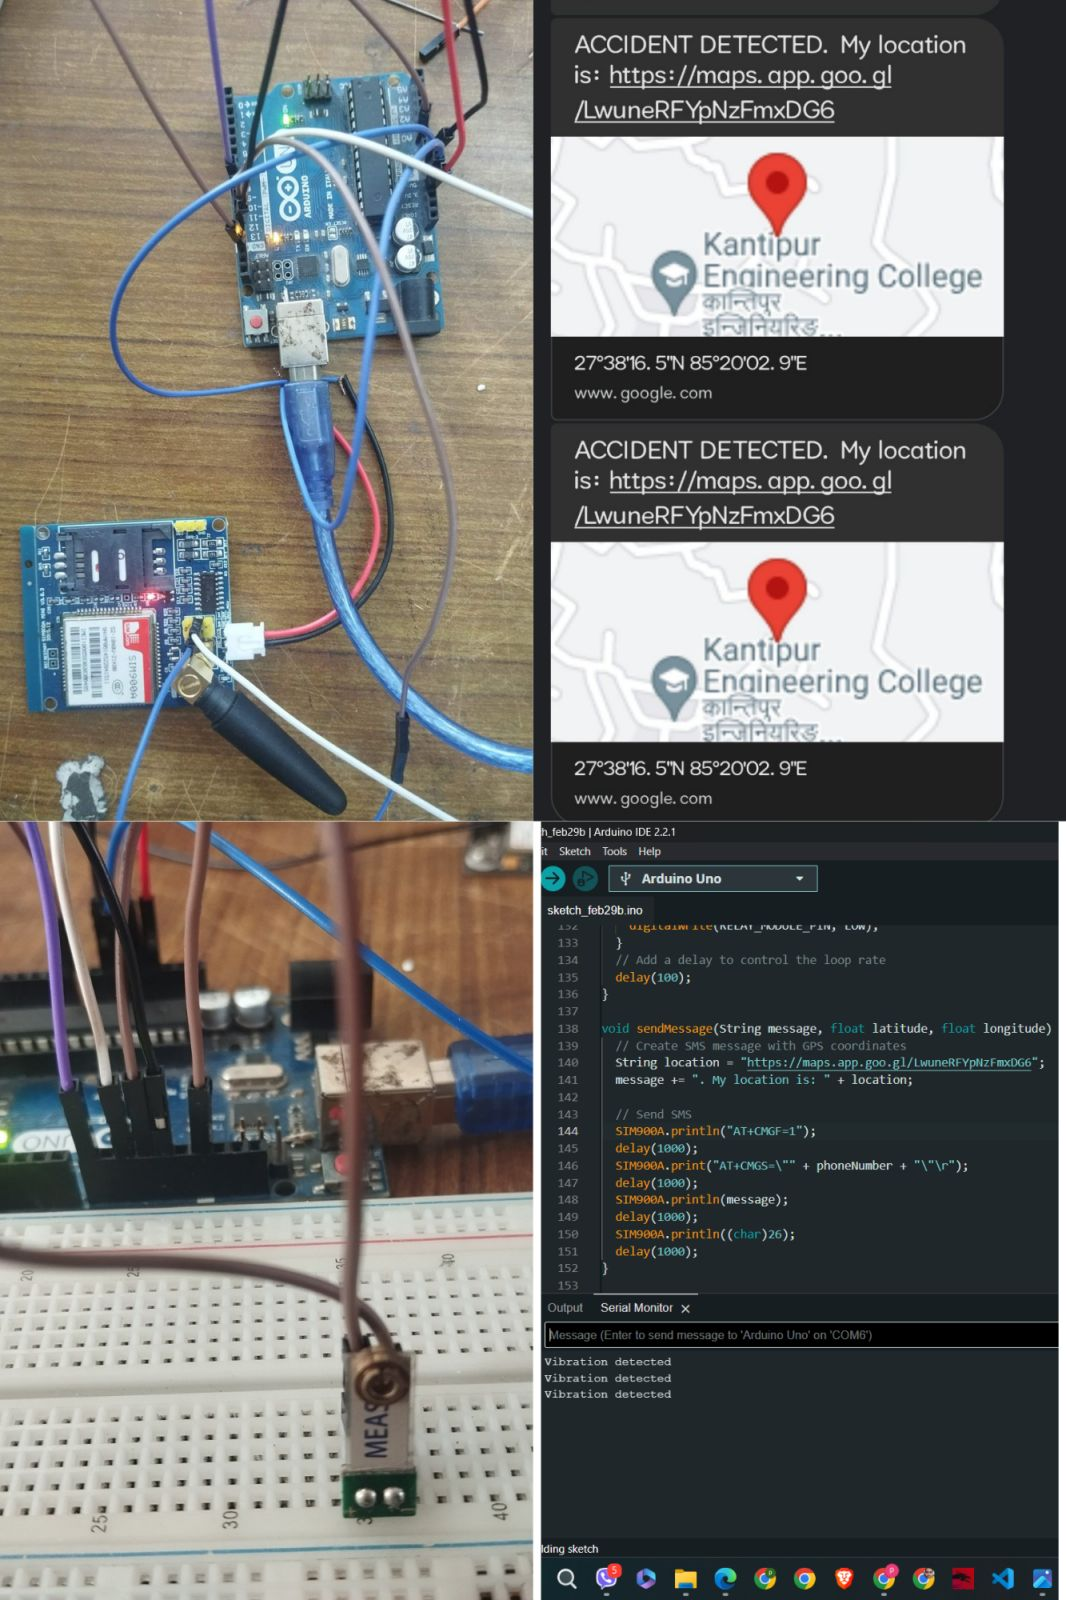
\includegraphics[height=15cm,width=15cm]{viber_image_2024-02-29_14-57-39-711.jpg}
\end{figure}
\end{document}